\documentclass[../main.tex]{subfiles}
\graphicspath{{\subfix{../images/}}} % Pfad zu den Bilddateien anpassen

\begin{document}

\section{Einleitung}

\textbf{Hello world!} % Beispiel für fettgedruckten Text

% Beispiel für eine Abbildung
\begin{figure}[h]
    \centering
    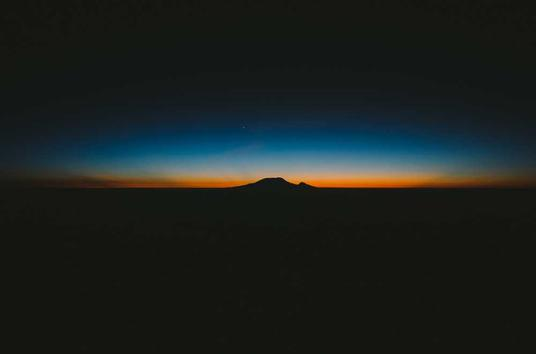
\includegraphics[width=3cm]{images/picsum lorem.jpg} % Pfad zur Abbildung
    \caption{Overleaf picsum lorem} % Beschriftung der Abbildung
    \label{fig:picsum_lorem} % Label für die Abbildung
\end{figure}

Lorem Ipsum bla\autocite[10]{smith2018} bla bla. As stated by bla bla bla. % Beispiel für eine Zitierung

Hier benutzen wir abkürzungen wir \gls{ml} und \gls{ai}.\\ % Beispiel für die Verwendung von Abkürzungen
Außerdem ist es jetzt hier \gls{ml} abgekürzt

Ein Beispieltext mit einem Gesetzeszitat \lawcite[§ 164 Absatz 1 Satz 1]{aktg1965}. % Beispiel für ein Gesetzeszitat

Test Test \autocite[15-27]{johnson2020} % Weitere Zitierung

\medskip

% Beispiel für eine Tabelle
\begin{table}[h]
    \centering
    \begin{tabular}{cc}
        Test & Test2\\
        Test3 & Test4\\
    \end{tabular}
    \caption{Beispiel-Tabelle} % Beschriftung der Tabelle
    \label{tab:example_table} % Label für die Tabelle
\end{table}

\end{document}
